\documentclass[11pt, a4paper]{article}
\usepackage{amsmath, amssymb, titling}
\usepackage[margin=2.5cm]{geometry}
\usepackage[colorlinks=true, linkcolor=black, urlcolor=black, citecolor=black]{hyperref}
\usepackage{graphicx}
\usepackage{float}

% \usepackage{minted}
\usepackage{xcolor}

\renewcommand\maketitlehooka{\null\mbox{}\vfill}
\renewcommand\maketitlehookd{\vfill\null}

\title{Satellite Orbit Control \\ HW2}
\author{Almog Dobrescu\\\\ID 214254252}

\begin{document}

\maketitle

\thispagestyle{empty}
\newpage
\setcounter{page}{1}

\tableofcontents
\vfil
\listoffigures
\newpage

\section{Given}
\begin{equation*}
    \begin{matrix}
        T_1=100\left[min\right] = 6\cdot10^3\left[sec\right] && T_2 = T_1 = 6\cdot10^3\left[sec\right] \\
        e_1 = 0 && e_2 = 0 \\
        a_1 = \sqrt[3]{\frac{\mu T_1^2}{4\pi^2}} = 7.1366\cdot10^3\left[km\right] && a_2 = a_1 = 7.1366\cdot10^3\left[km\right]
    \end{matrix}\\
\end{equation*}
\begin{equation*}
    \alpha=\Delta i = 0.01^\circ
\end{equation*}
In CW frame with origin at Satellite \#1 and at $t=0$:
\begin{equation*}
    \begin{matrix}
    \begin{pmatrix}
        x_2(0)=0 \\ y_2(0)=-1 \\ z_2(0)=1
    \end{pmatrix}\left[km\right] &&
    \begin{pmatrix}
        \dot{x}_2(0)=?? \\ \dot{y}_2(0) = ?? \\ \dot{z}_2(0)<0
    \end{pmatrix}
    \end{matrix}
\end{equation*}
Desired:
\begin{equation*}
    \begin{matrix}
    \begin{pmatrix}
        x_2(t_1)=0 \\ y_2(t_1)=0 \\ z_2(t_1)=0
    \end{pmatrix} &&
    \begin{pmatrix}
        \dot{x}_2(t_1)=0 \\ \dot{y}_2(t_1)=0 \\ \dot{z}_2(t_1)=0
    \end{pmatrix}
    \end{matrix}
\end{equation*}
Limitations:
\begin{equation*}
    \Delta v = t \begin{pmatrix}
        0\\
        \Delta v_y\\
        \Delta v_z
    \end{pmatrix}
\end{equation*}

\section{A}
General equations of motion in CW fram:
\begin{equation}
    \left\{\begin{array}{l}
        \ddot{x}-2n\dot{y}-3n^2x=f_x\\
        \ddot{y}+2n\dot{x}=f_y\\
        \ddot{z}+n^2z=f_z
    \end{array}\right.
\end{equation}
The velocities:
\begin{equation}
    \left\{\begin{array}{l}
        u_x = \dot{x}-ny(t)\\
        u_y = \dot{y}+nx(t)\\
        u_z = \dot{z}
    \end{array}\right.
\end{equation}
The solution without external forces (i.e. $\vec{f}=\vec{0}$):
\begin{equation}
    \left\{\begin{array}{l}
        \displaystyle x(t) = \left(4-3\cos(nt)\right)\cdot x_0 + \frac{\dot{x}_0}{n}\sin(nt)+\frac{2}{n}\left(1-\cos(nt)\right)\cdot\dot{y}_0 \\
        \displaystyle y(t) = 6\left(\sin(nt)-nt\right)\cdot x_0 + y_0 + \frac{2}{n}\left(\cos(nt)-1\right)\cdot\dot{x}_0 + \left(4\sin(nt)-3nt\right)\frac{\dot{y}_0}{n} \\
        \displaystyle z(t)=z_0\cos(nt)+\frac{\dot{z}_0}{n}\sin(nt)
    \end{array}\right.
\end{equation}
Because the two satellite have the same period, then in CW fram, it is a no-drift orbit:
\begin{equation}
    \begin{array}{l}
        \dot{y}_0=-2nx_0
    \end{array}
\end{equation}
From the angle between the plains we can claculate $\dot{z}_2(0)$:
\begin{align}
    \tan\alpha &= \frac{z_{max}}{a_1} = \frac{\displaystyle\sqrt{z_2(0)^2+\left(\frac{\dot{z}_2(0)}{n}\right)^2}}{a_1} \\
    \frac{\dot{z}_2(0)}{n} &= \underbrace{-}_{\displaystyle\dot{z}_2(0)<0}\sqrt{\left(a_1\cdot\tan(\alpha)\right)^2-z_2(0)^2} \\
    \frac{\dot{z}_2(0)}{n} &= -0.7426;
\end{align}
Because we can't apply a velocity pulse in the x direction, $\dot{x}_2(0) = 0$. The CW frame is therefor:
\begin{equation}
    \begin{matrix}
    \begin{pmatrix}
        x_2(0)=0 \\ y_2(0)=-1 \\ z_2(0)=1
    \end{pmatrix}\left[km\right] &&
    \begin{pmatrix}
        \dot{x}_2(0)=0 \\ \dot{y}_2(0) =0 \\ \dot{z}_2(0)=-0.74267\cdot n
    \end{pmatrix}\left[\displaystyle\frac{km}{sec}\right]
    \end{matrix}
\end{equation}
% So the equations of motion becomes:
% \begin{equation}
%     \left\{\begin{array}{l}
%         \displaystyle x(t) = x_0\cos(nt) + \frac{\dot{x}_0}{n}\sin(nt) \\
%         \displaystyle y(t) = y_0 + \frac{2}{n}\left(\cos(nt)-1\right)\cdot\dot{x}_0 -2x_0\sin(nt) \\
%         \displaystyle z(t)=z_0\cos(nt)+\frac{\dot{z}_0}{n}\sin(nt)
%     \end{array}\right.
% \end{equation}
%\begin{equation}
%     \left\{\begin{array}{l}
%         \displaystyle\dot{x}(t) = -nx_0\sin(nt) + \dot{x}_0\cos(nt) \\
%         \displaystyle\dot{y}(t) = -\frac{2\dot{x}_0}{n}\left(n\sin(nt)+1\right)-2nx_0\cos(nt) \\
%         \dot{z}(t) = -nz_0\sin(nt) + \dot{z}_0\cos(nt)
%     \end{array}\right.
% \end{equation}

% The required maneuver time is the time required for the position in the \emph{z} direction to become zero:
% \begin{align}
%     z_0\cos(nt)+\frac{\dot{z}_0}{n}\sin(nt) &= 0 \\
%     \cos(nt)+\frac{\dot{z}_0}{n}\sin(nt) &= 0 \\
%     \sqrt{1^2+\frac{\dot{z}}{n}}\cos\left(nt + \arctan\left(\frac{\displaystyle -\frac{\dot{z}_0}{n}}{1}\right)\right) = 0 \\
%     nt +\arctan\left(\frac{\displaystyle -\frac{\dot{z}_0}{n}}{1}\right) = \frac{\pi}{2} + \pi k
% \end{align}

The CW equations in state-space form:
\begin{equation}
    \begin{matrix}
        \text{x-y plane:} && \text{z-direction:} \\
        \begin{matrix}
            x1 = x \\
            x2 = \dot{x}
        \end{matrix} && z1 = z \\
        \begin{matrix}
            y1 = y \\
            y2 = \dot{y}
        \end{matrix} && z2 = \dot{z}
    \end{matrix}
\end{equation}
The homogeneous solution:
\begin{equation}
    \vec{x}(t) = \Phi_{(t,t_0)}\vec{x}_0
\end{equation}
\begin{equation}
    \begin{array}{l}
        \text{x-y plane:} \\
        \Phi_{(t,t_0)} = \left(\begin{array}{cc|cc}
            4-3\cos(n\tau) & 0 &\displaystyle \frac{1}{n}\sin(n\tau) &\displaystyle \frac{2}{n}\left(1-\cos(n\tau)\right) \\ 
            6\left(\sin(n\tau)-n\tau\right) & 1 &\displaystyle \frac{2}{n}\left(\cos(n\tau)-1\right) &\displaystyle \frac{1}{n}\left(4\sin(n\tau)-3n\tau\right)\\ &&& \\ \hline &&& \\
            3n\sin(n\tau) & 0 & \cos(n\tau) & 2\sin(n\tau) \\
            6n\left(\cos(n\tau)-1\right) & 0 & -2\sin(n\tau) & 4\cos(n\tau)-3 
        % \Phi_{(t,t_0)} = \left(\begin{array}{cc|cc}
        %     \cos(n\tau) & 0 &\displaystyle \frac{1}{n}\sin(n\tau) & 0 \\ 
        %     -2n\cos(n\tau) & 1 &\displaystyle \frac{2}{n}\left(\cos(n\tau)-1\right) &0\\ &&& \\ \hline &&& \\
        %     -n\sin(n\tau) & 0 & \cos(n\tau) & 0 \\
        %     -2n\cos(n\tau) & 0 & \displaystyle-\frac{2}{n}\left(n\sin(n\tau)+1\right) & 0 
        \end{array}\right) = \begin{pmatrix}
            \Phi_{11(t,t_0)} & \Phi_{12(t,t_0)} \\
            \Phi_{21(t,t_0)} & \Phi_{22(t,t_0)}
        \end{pmatrix} \\ \\ 
    \text{z-direction:} \\
    \Phi_{(t,t_0)} = \begin{pmatrix}
        \cos(n\tau) & \displaystyle\frac{1}{n}\sin(n\tau) \\
        -n\sin(n\tau) & \cos(n\tau)
    \end{pmatrix}
    \end{array}
\end{equation}
Where:
\begin{equation*}
    \tau = t-t_0
\end{equation*}
Desired:
\begin{equation}
    \begin{matrix}
        \begin{pmatrix}
            x1\\
            y1\\
            x2\\
            y2
        \end{pmatrix}(t_1) & = & \vec{0} \\\\
        \begin{pmatrix}
            z1\\
            z2
        \end{pmatrix}(t_1) & = & \vec{0}
    \end{matrix}
\end{equation}
% As the lecture shows, for a maneuver with $\Delta v_x = 0$, the maneuver time equals one orbital period $t_1 = T_1$. The transition matrix quadrants for $n\tau = 2\pi$:
% \begin{equation}
%     \begin{array}{lcl}
%         \Phi_{11}=\begin{pmatrix}
%             1 & 0 \\
%             -2n & 1
%         \end{pmatrix} && \Phi_{12}=\begin{pmatrix}
%             0 & 0 \\
%             0 & 0
%         \end{pmatrix} \\\\
%         \Phi_{21}=\begin{pmatrix}
%             0 & 0 \\
%             -2n & 0
%         \end{pmatrix} && \Phi_{22}=\begin{pmatrix}
%             1 & 0 \\
%             \displaystyle-\frac{2}{n} & 0
%         \end{pmatrix}
%     \end{array}
% \end{equation}
The required velocity components are found from the first 2 lines of $\vec{x}(t_1)=\Phi_(t_1,0)\vec{x(0)}$:
\begin{equation}
    \begin{pmatrix}
        x_{(t_1)}\\y_{(t_1)}
    \end{pmatrix} = \vec{0} = \Phi_{11(t_1, 0)}\begin{pmatrix}
        x(0)\\y(0)
    \end{pmatrix} + \Phi_{12(t_1,0)}\begin{pmatrix}
        \dot{x}_{req} \\
        \dot{y}_{req}
    \end{pmatrix}
\end{equation}
\begin{equation*}
    \Downarrow
\end{equation*}
\begin{equation}
    \begin{pmatrix}
        \dot{x}_{req} \\
        \dot{y}_{req}
    \end{pmatrix} = -\Phi_{12(t_1,0)}^{-1}\Phi_{11(t_1,0)}\begin{pmatrix}
        x(0)\\y(0)
    \end{pmatrix} \equiv \mathbf{C}^*_{(t_1,0)} \begin{pmatrix}
        x(0)\\y(0)
    \end{pmatrix}
\end{equation}
The terminal velocity is determined from the last two rows of $\vec{x}(t_1)=\Phi_(t_1,0)\vec{x(0)}$:
\begin{equation}
    \begin{pmatrix}
        \dot{x}_{(t_1)}\\\dot{y}_{(t_1)}
    \end{pmatrix} = \Phi_{21(t_1,0)}\begin{pmatrix}
        x(0)\\y(0)
    \end{pmatrix} + \Phi_{22(t_1,0)}\begin{pmatrix}
        \dot{x}_{req} \\
        \dot{y}_{req}
    \end{pmatrix}
\end{equation}
Because we can't apply a velocity pulse in the x direction, we set $\dot{x}_{t_1}$ to be zero. Using \emph{MatLab}, the first equation after substituting the initial conditions is:
\begin{equation}
    \frac{\displaystyle2\pi\left(\cos\left(\frac{\pi\tau}{3000}\right)-1\right)}{\displaystyle24000\cos\left(\frac{\pi\tau}{3000}\right)+3\tau\pi\sin\left(\frac{\pi\tau}{3000}\right)-24000} = 0
\end{equation}
\begin{align}
    \cos\left(\frac{\pi\tau}{3000}\right) &= 1 \\
    \frac{\pi\tau}{3000} &= 2\pi \\
    \pi\tau &= 6000\pi \\
    \tau &= 6000
\end{align}
\\
$$\colorbox{yellow}{$t_1 = \tau = 6000\left[sec\right]$\hspace{1cm}(exactly on period)}$$

\section{B}
\subsection{x-y plane}
The first pulse is the difference between the required velocity and the initial velocity:
\begin{equation}
    \begin{pmatrix}
        \Delta v_{x1} \\ \Delta v_{y1}
    \end{pmatrix} = \begin{pmatrix}
        \dot{x}_{req} \\ \dot{y}_{req}
    \end{pmatrix} - \begin{pmatrix}
        \dot{x}_{(t_1)} \\ \dot{y}_{(t_1)}
    \end{pmatrix}
\end{equation}
\begin{equation}
    \begin{array}{ll}
        \Phi_{11} = \begin{pmatrix}
            1 & 0 \\
            -12\pi & 1
        \end{pmatrix} & \Phi_{12} = \begin{pmatrix}
            0 & 0 \\
            0 & -18000
        \end{pmatrix} \\
        \Phi_{21} = \begin{pmatrix}
            0 & 0 \\
            0 & 0
        \end{pmatrix} &
        \Phi_{22} = \begin{pmatrix}
            1 & 0 \\
            0 & 1
        \end{pmatrix}
    \end{array}
\end{equation}
Since $\left|\Phi_{12}\right| = 0$, we can't use the state space. let's look at the CW equations of motion for no-drift orbti:
% \begin{equation}
%     \begin{matrix}
%         \left\{\begin{array}{l}
%             x_{(t)} = \displaystyle\frac{\dot{x}_0}{n}\sin(nt) + x_0\cos(nt)\\
%             y_{(t)} = \displaystyle y_0 + \frac{2\dot{x}_0}{n}\left(\cos(nt)-1\right) -2x_0\sin(nt) \\
%             z_{(t)} = \displaystyle z_0 \cos(nt) + \frac{\dot{z}_0}{n}\sin(nt)
%         \end{array}\right. \\\\
%         \left\{\begin{array}{l}
%             \displaystyle\dot{x}_{(t)} = -nx_0\sin(nt) + \dot{x}_0\cos(nt) \\
%             \displaystyle\dot{y}_{(t)} = -\frac{2\dot{x}_0}{n}\left(n\sin(nt)+1\right)-2nx_0\cos(nt) \\
%             \dot{z}_{(t)} = -nz_0\sin(nt) + \dot{z}_0\cos(nt)
%         \end{array}\right. \\\\
%         \begin{matrix}
%             x_0 = 0 & y_0 = -1 & z_0 = 1 & x_{(t_1)} = 0 & y_{(t_1)} = 0 & t_1 = 6000 & nt = 2\pi% & \dot{x}_0 = 0 & \dot{y}_0 = 0 & \dot{z}_0 = -0.7426
%         \end{matrix}
%     \end{matrix}
% \end{equation}
% Calculating the required velocity in the \emph{y} direction:
% \begin{equation}
%     y_{(t_1)} = 0 = \displaystyle -1 + \frac{2\dot{x}_0}{n}\left(\cos(2\pi)-1\right) 
% \end{equation}
\begin{equation}
    \begin{matrix}
        \left\{\begin{array}{l}
            \displaystyle x_{(t)} = \left(4-3\cos(nt)\right)\cdot x_0 + \frac{\dot{x}_0}{n}\sin(nt)+\frac{2}{n}\left(1-\cos(nt)\right)\cdot\dot{y}_0 \\
            \displaystyle y_{(t)} = 6\left(\sin(nt)-nt\right)\cdot x_0 + y_0 + \frac{2}{n}\left(\cos(nt)-1\right)\cdot\dot{x}_0 + \left(4\sin(nt)-3nt\right)\frac{\dot{y}_0}{n} \\
            \displaystyle z_{(t)}=z_0\cos(nt)+\frac{\dot{z}_0}{n}\sin(nt)
        \end{array}\right. \\\\
        \left\{\begin{array}{l}
            \displaystyle\dot{x}_{(t)} = 3nx_0\sin(nt) + \dot{x}_0\cos(nt) +2\dot{y}_0\sin(nt) \\
            \displaystyle\dot{y}_{(t)} = 6nx_0\left(\cos(nt)-1\right) -2\dot{x}_0\sin(nt) + \dot{y}_0\left(4\cos(nt)-3\right) \\
            \dot{z}_{(t)} = -nz_0\sin(nt)+\dot{z}_0\cos(nt)
        \end{array}\right. \\\\
        \begin{matrix}
            x_0 = 0 & y_0 = -1 & z_0 = 1 & x_{(t_1)} = 0 & y_{(t_1)} = 0 & t_1 = 6000 & nt = 2\pi% & \dot{x}_0 = 0 & \dot{y}_0 = 0 & \dot{z}_0 = -0.7426
        \end{matrix}
    \end{matrix}
\end{equation}
From the position at the \emph{y} direction:
\begin{equation}
    \begin{array}{c}
        \displaystyle y_{(t_1)} = 0 = 6\left(\sin(2\pi)-2\pi\right)\cdot 0 + -1 + \frac{2}{n}\left(\cos(2\pi)-1\right)\cdot0 + \left(4\sin(2\pi)-3\cdot2\pi\right)\frac{\dot{y}_{req}}{n} \\
        \displaystyle0 = -1 + \left(-3\cdot2\pi\right)\frac{\dot{y}_0}{n} \\
        \displaystyle\dot{y}_{req} = -\frac{n}{6\pi} = -5.5556\cdot10^{-5} \left[\frac{km}{sec}\right] \\
        \Downarrow \\
        \begin{pmatrix}
            \Delta v_{x1} \\ \Delta v_{y1}
        \end{pmatrix} = \begin{pmatrix}
            \dot{x}_{req} \\ \dot{y}_{req}
        \end{pmatrix} - \begin{pmatrix}
            \dot{x}_{(0)} \\ \dot{y}_{(0)}
        \end{pmatrix} = \begin{pmatrix}
            0 \\ -5.5556\cdot10^{-5}
        \end{pmatrix} - \begin{pmatrix}
            0 \\ 0
        \end{pmatrix} \\
        \Downarrow \\
        \colorbox{yellow}{$ \begin{pmatrix}
            \Delta v_{x1} \\ \Delta v_{y1}
        \end{pmatrix}_{(t=0)} = \begin{pmatrix}
            0 \\ -5.5556
        \end{pmatrix}\cdot10^{-5}\left[\frac{km}{sec}\right]$}
    \end{array}
\end{equation}
For a rendezvous maneuver, a terminal velocity pulse is applied such that the terminal velocity is zero:
\begin{align}
    \begin{pmatrix}
        \Delta v_{x2} \\ \Delta v_{y2}
    \end{pmatrix} &= -\begin{pmatrix}
        \dot{x}_{(t_1)}\\\dot{y}_{(t_1)}
    \end{pmatrix} \\
    &= - \begin{pmatrix}
        3nx_0\sin(nt) + \dot{x}_0\cos(nt) +2\dot{y}_0\sin(nt) \\ 6nx_0\left(\cos(nt)-1\right) -2\dot{x}_0\sin(nt) + \dot{y}_0\left(4\cos(nt)-3\right) 
    \end{pmatrix} \\
    &= - \begin{pmatrix}
        -2\cdot5.5556\cdot10^{-5}\cdot\sin(2\pi) \\
        -5.5556\cdot10^{-5}\cdot\left(4\cos(2\pi)-3\right) 
    \end{pmatrix} \\
    &= - \begin{pmatrix}
        0 \\
        -5.5556\cdot10^{-5}
    \end{pmatrix}
\end{align}
\begin{equation*}
    \begin{array}{c}
        \Downarrow\\
        \colorbox{yellow}{$ \begin{pmatrix}
            \Delta v_{x2} \\ \Delta v_{y2}
        \end{pmatrix}_{(t=6000[sec])} = \begin{pmatrix}
            0 \\ 5.5556
        \end{pmatrix}\cdot10^{-5}\left[\frac{km}{sec}\right]$}
    \end{array}
\end{equation*}

\subsection{z direction}
Since $t_f (t_1)$ is bigger than half of a period, there is no need for an initial pulse. Let's find the time until $z = 0$:
\begin{align}
    \displaystyle z_{(t)} = 0 &= z_0\cos(nt)+\frac{\dot{z}_0}{n}\sin(nt) \\
    0 &= 1\cdot\cos(nt)+\frac{-0.74267\cdot n}{n}\sin(nt) \\
    0 &= \cos(nt) -0.74267\sin(nt)
\end{align}
\begin{equation*}
    \begin{matrix}
        a\sin(x) +b\cos(x) = \displaystyle\sqrt{a^2+b^2}\sin(x+\varphi) \\
        \varphi = \displaystyle\arctan\left(\frac{b}{a}\right)
    \end{matrix}
\end{equation*}
\begin{equation}
    1.2456\sin(nt+2.2096) = 0 
\end{equation}
\begin{equation}
    nt+2.2096 = \pi\cdot k
\end{equation}
\begin{equation}
    nt = 0.9320
\end{equation}
\begin{equation}
    t_{(z=0)} = 889.9874[sec]
\end{equation}
So the velocity in the \emph{z} direction when $z=0$:
\begin{align}
    \dot{z}_{(t)} &= -nz_0\sin(nt)+\dot{z}_0\cos(nt) \\
    \dot{z}_{(z=0)} &= -n\cdot1\cdot\sin(0.9320)-0.74267\cdot n\cos(0.9320) 
\end{align}
\begin{equation*}
    \displaystyle\dot{z}_{(z=0)} = -0.0013\left[\frac{km}{sec}\right]
\end{equation*}
\begin{equation*}
    \Downarrow
\end{equation*}
\begin{equation*}
    \colorbox{yellow}{$\Delta v_{z1(t=889.9874[sec])} = -\dot{z}_{z=0} = 0.0013\left[\frac{km}{sec}\right]$}
\end{equation*}

\section{C}
\begin{figure}[H]
    \centering
    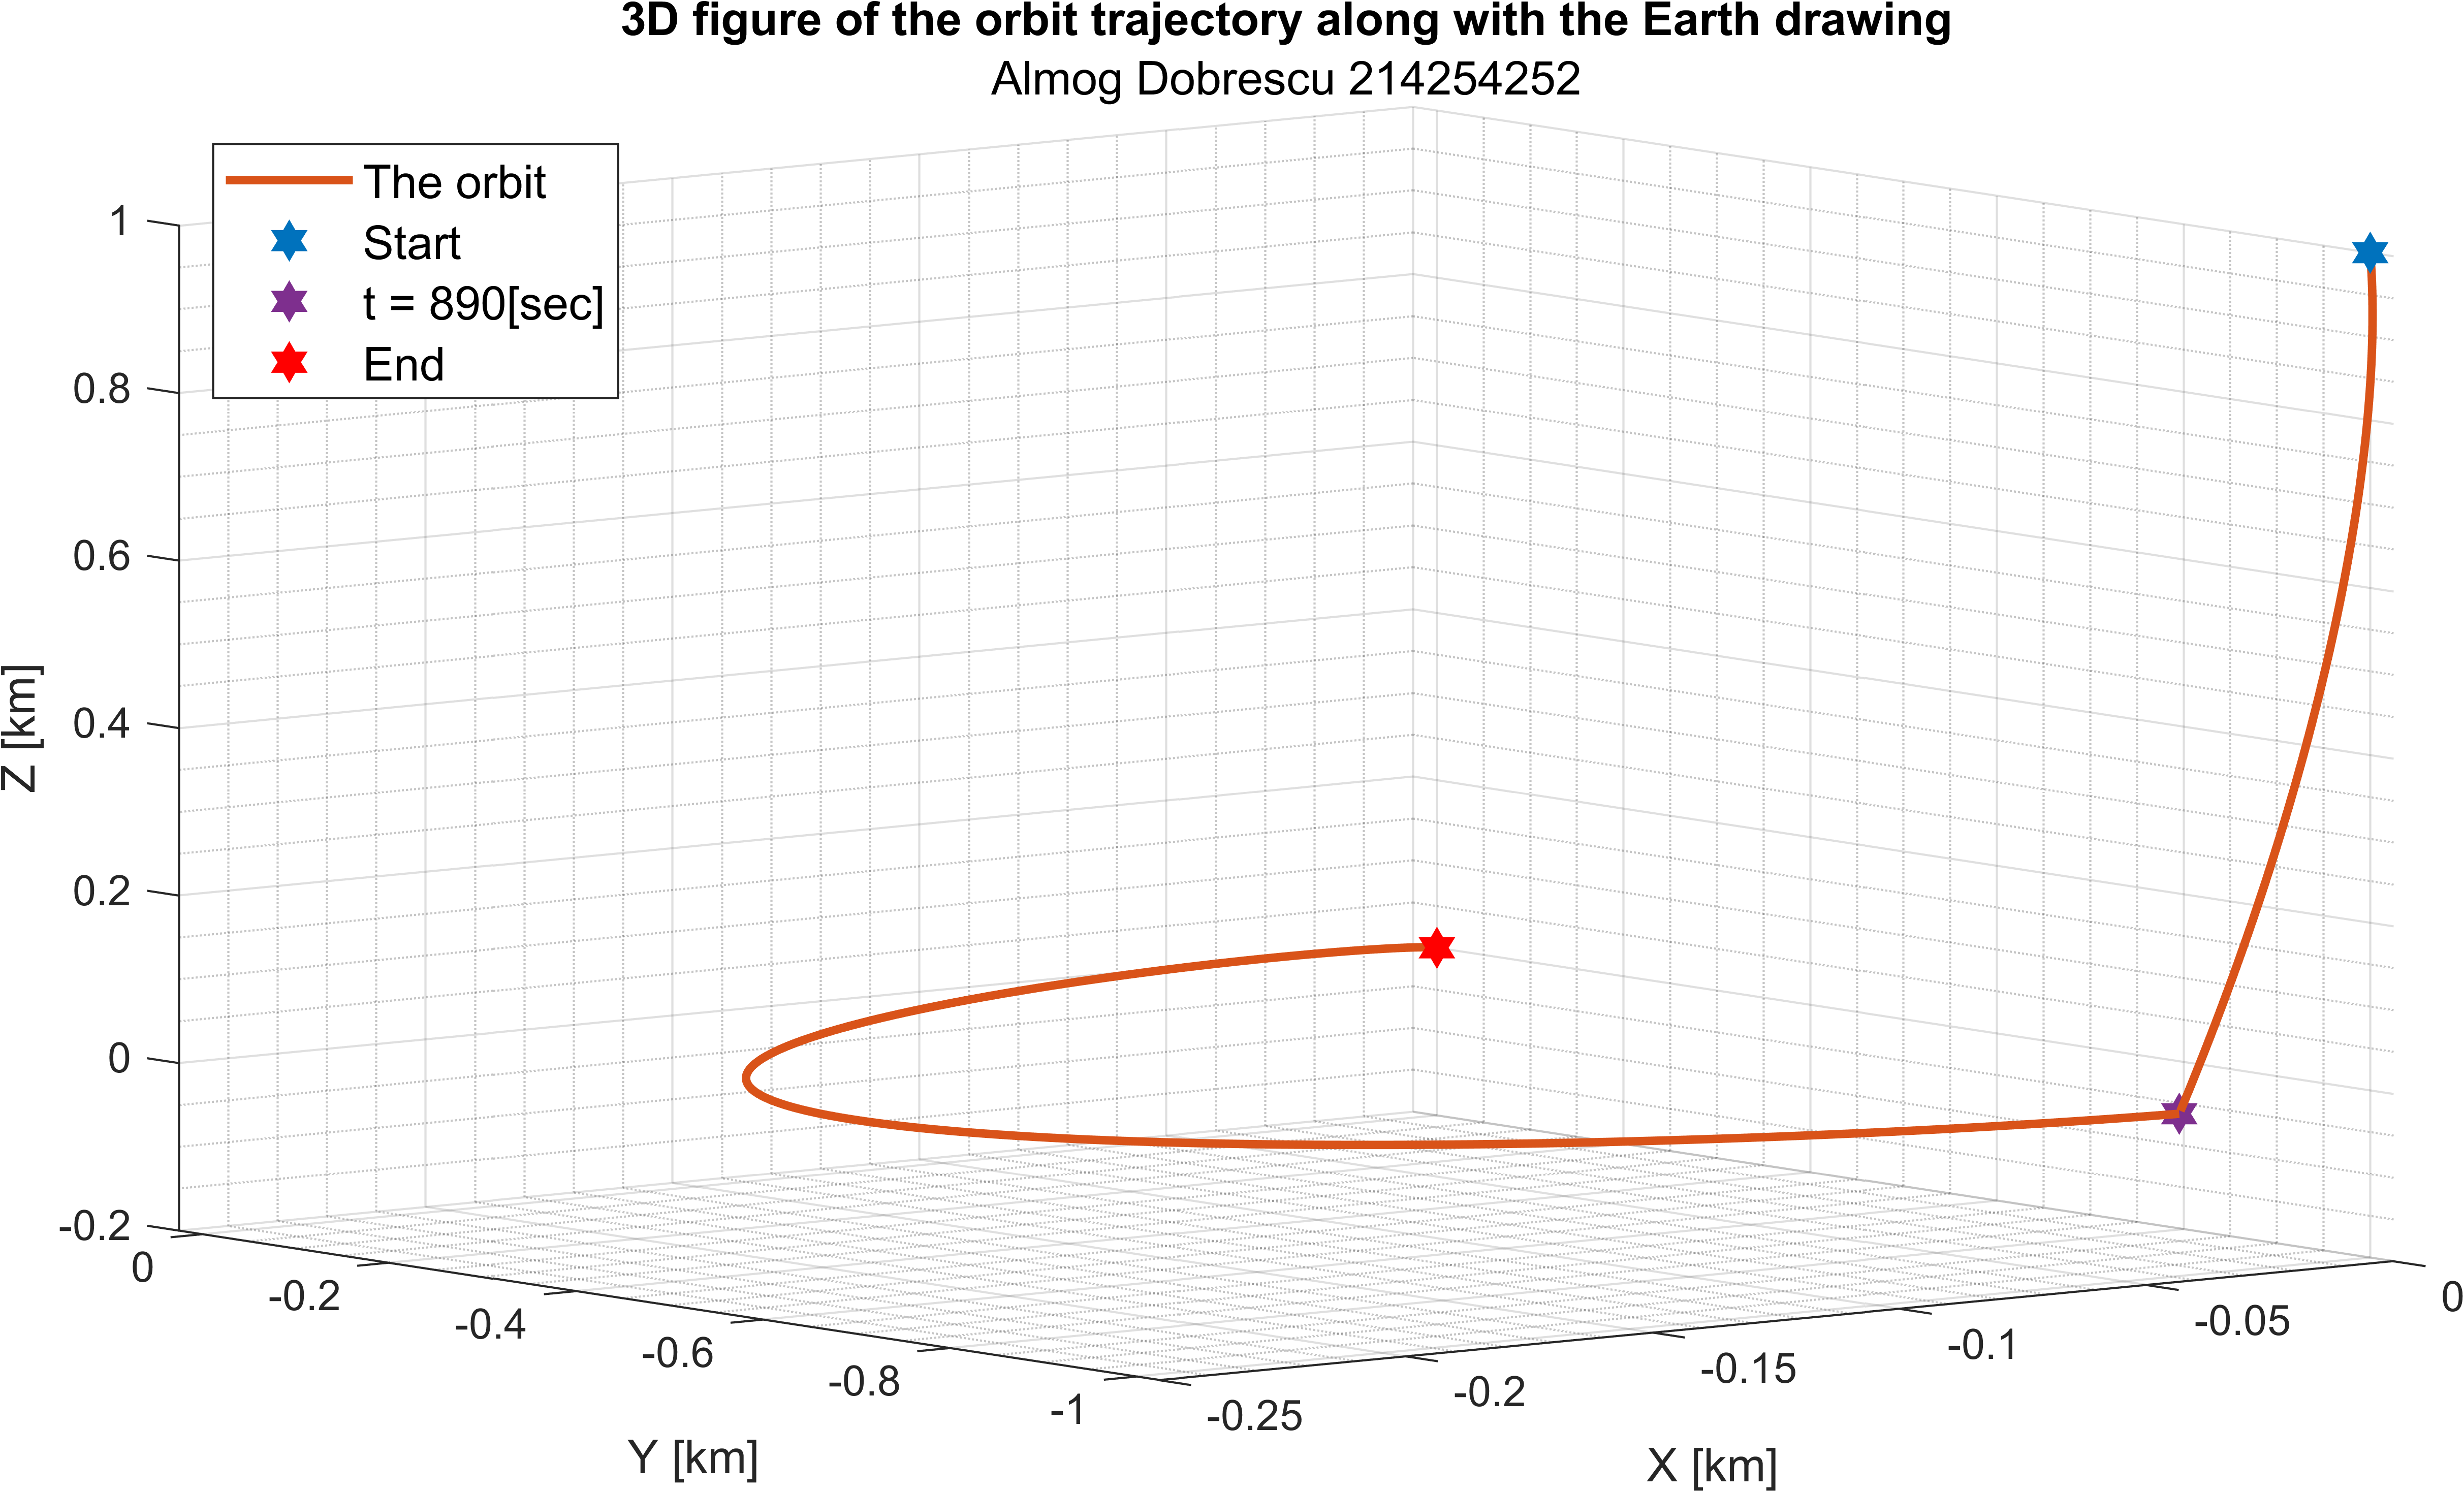
\includegraphics[width=0.9\textwidth]{images/3D plot.png}
    \caption{3D figure of the orbit trajectory along with the Earth drawing}
    \label{fig:3D-plot}
\end{figure}

\section{D}
\begin{equation*}
    \begin{matrix}
        \left(\begin{array}{c}
            \Delta x_m \\ \Delta y_m \\ \Delta z_m
        \end{array}\right) = \left(\begin{array}{c}
            \pm 1 \\
            \pm 1 \\
            \pm 1
        \end{array}\right)\cdot10^{-3}\left[km\right] &&&& \left(\begin{array}{c}
            \Delta \dot{x}_m \\ \Delta \dot{y}_m \\ \Delta \dot{z}_m
        \end{array}\right) = \left(\begin{array}{c}
            \pm 1 \\
            \pm 1 \\
            \pm 1
        \end{array}\right)\displaystyle\cdot10^{-5}\left[\frac{km}{sec}\right] \\
        &&\tau = 6000&& 
    \end{matrix}
\end{equation*}
The worst case miss distance is the sum of the absolute values:
\begin{equation}
    \left\{\begin{array}{l}
        \displaystyle\left.\Delta x_f\right|_\text{worst case} = \left|\Delta x_m\left(4-3\cos(n\tau)\right)\right| + \left|\frac{\Delta\dot{x}_m}{n}\sin(n\tau)\right| + \left|\frac{2\Delta\dot{y}_m}{n}\left(1-\cos(n\tau)\right)\right| \\
        \displaystyle\left.\Delta y_f\right|_\text{worst case} = \left|6\Delta x_m\left(\sin(n\tau)-n\tau\right)\right| + \left|\Delta y_m\right| + \left|\frac{2\Delta\dot{x}_0}{n}\left(\cos(n\tau)-1\right)\right| + \left|\frac{\Delta\dot{y}_m}{n}\left(4\sin(n\tau)-3n\tau\right)\right| \\
        \displaystyle\left.\Delta z_f\right|_\text{worst case} = \left|\Delta z_m\cos(n\tau)\right| + \left|\frac{\Delta\dot{z}_m}{n}\sin(n\tau)\right|
    \end{array}\right.
\end{equation}
\begin{equation*}
    \Downarrow
\end{equation*}
\begin{equation}
    \colorbox{yellow}{$\left\{\begin{array}{l}
        \displaystyle\left.\Delta x_f\right|_\text{worst case} = 0.001 \\
        \displaystyle\left.\Delta y_f\right|_\text{worst case} = 0.2187 \\ 
        \displaystyle\left.\Delta z_f\right|_\text{worst case} = 0.001
    \end{array}\right.$}
\end{equation}




\end{document}